\section{Theoretical framework}

\subsection{Graph theory}
This section contains definitions, notation and concepts related to Graph Theory according
to \cite{graph_theory:2010}.
Graph theory deals with connection amongst vertices by edges. \\
Graphs are the foundation of many day to day processes and concepts, as they provide a convenient
and intuitive way of representing objects.

\subsubsection{Simple graphs}
A \textbf{simple graph} \textit{G} consists of a non-empty finite set \textit{V(G)} of elements called \textbf{vertices}
(or \textbf{nodes}), and a finite set \textit{E(G)} of distinct unordered pairs of distinct elements of \textit{V(G)}
called \textbf{edges}. We call \textit{V(G)} the \textbf{vertices set} and \textit{E(G)} the \textbf{edge set} of G.
An edge $\{\textit{v}, \textit{w}\}$ is said to \textbf{join} the vertices v and w, and is usually abbreviated to vw. For example, Figure~\ref{fig:simple_graph} represents the simple graph G whose vertex set \textit{V(G)} is $\{\textit{u}, \textit{v}, \textit{w}, \textit{z}\}$, and whose
edge set \textit{E(G)} consists of the edges \textit{uv}, \textit{uw}, \textit{vw} and \textit{wz}. 

\begin{figure}[H]
    \centering
    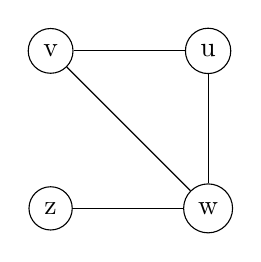
\begin{tikzpicture}
      % Disegno dei nodi
      \node[circle, draw] (v) at (0,0) {v};
      \node[circle, draw] (u) at (2,0) {u};
      \node[circle, draw] (w) at (2,-2) {w};
      \node[circle, draw] (z) at (0,-2) {z};
      
      % Disegno degli archi
      \draw (u) -- (v);
      \draw (u) -- (w);
      \draw (v) -- (w);
      \draw (w) -- (z);
    \end{tikzpicture}
    \caption{}
    \label{fig:simple_graph}
\end{figure}

\subsubsection{Adjacency}
We say that two vertices \textit{v} and \textit{w} of a graph \textit{G} are \textbf{adjacent} if there is an edge \textit{vw} joining them, and the vertices \textit{v} and \textit{w} are then \textbf{incident} with such an edge.
Similarly, two distinct edges \textit{e} and \textit{f} are \textbf{adjacent} if they have a vertex in common (see Figure \ref{fig:adiacency}).

\begin{figure}[H]
    \centering
    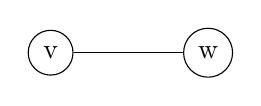
\begin{tikzpicture}
      % Primo grafo
      \node[circle, draw] (v) at (0,0) {v};
      \node[circle, draw] (w) at (2,0) {w};
      \draw (v) -- (w);
    \end{tikzpicture}
    \quad % Spazio tra i grafi
    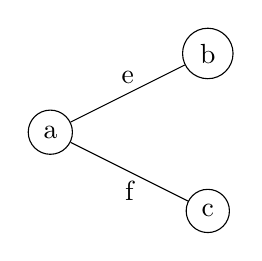
\begin{tikzpicture}
      % Secondo grafo
      \node[circle, draw] (a) at (0,0) {a};
      \node[circle, draw] (b) at (2,1) {b};
      \node[circle, draw] (c) at (2,-1) {c};
      \draw (a) -- node[above] {e} (b);
      \draw (a) -- node[below] {f} (c);
    \end{tikzpicture}
    \caption{Adjacent vertices and adjacent edges}
    \label{fig:adiacency}
\end{figure}

\subsubsection{Matrix representations}
Although it is convenient to represent a graph by a diagram of points joined by lines,
such a representation may be unsuitable if we wish to store a large graph in a computer.
One way of storing a simple graph is involve matrices. \\
Let's consider a graph \textit{G} with \textit{n} vertices and \textit{m} edges. \\
An \textbf{adjacency matrix A} is the $n \times n$ matrix whose \textit{ij}-th entry is the number of edges joining vertex \textit{i} and vertex \textit{j}. \\
If, in addition, the edges are labelled $\{1, 2, \dots, m\}$, its \textbf{incidence matrix M} is the $n \times m$ matrix whose \textit{ij}-th entry is 1 if vertex \textit{i} is incident to edge \textit{j}, and 0 otherwise. \\
An example of this is given in Figure \ref{fig:matrix_representations}.

\begin{figure}[H]
    \centering
    \begin{minipage}{0.5\textwidth}
        \centering
        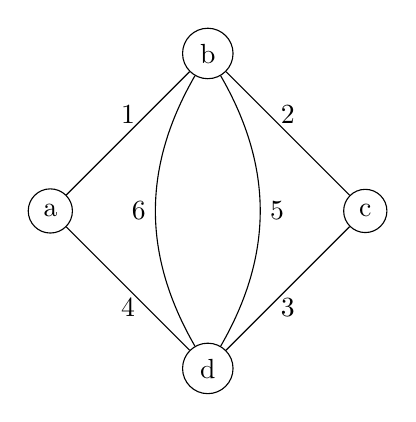
\begin{tikzpicture}
            % Nodi
            \node[circle, draw] (a) at (0,0) {a};
            \node[circle, draw] (b) at (2,2) {b};
            \node[circle, draw] (c) at (4,0) {c};
            \node[circle, draw] (d) at (2,-2) {d};
          
            % Archi
            \draw (a) edge node[pos=0.5, below] {4} (d);
            \draw (a) edge node[pos=0.5, above] {1} (b);
            \draw (b) edge[bend left] node[pos=0.5, right] {5} (d);
            \draw (b) edge[bend right] node[pos=0.5, left] {6} (d);
            \draw (b) edge node[pos=0.5, above] {2} (c);
            \draw (c) edge node[pos=0.5, below] {3} (d);
        \end{tikzpicture}
    \end{minipage}%
    \begin{minipage}{0.5\textwidth}
        \[
        A = \begin{bmatrix}
        0 & 1 & 0 & 1 \\
        1 & 0 & 1 & 2 \\
        0 & 1 & 0 & 1 \\
        1 & 2 & 1 & 0
        \end{bmatrix}
        \]
        
        \[
        M = \begin{bmatrix}
        1 & 0 & 0 & 1 & 0 & 0 \\
        1 & 1 & 0 & 0 & 1 & 1 \\
        0 & 1 & 1 & 0 & 0 & 0 \\
        0 & 0 & 1 & 1 & 1 & 1
        \end{bmatrix}
        \]
    \end{minipage}
    \caption{Graph \textit{G} with its adjacency and incidence matrices}
    \label{fig:matrix_representations}
\end{figure}


\subsubsection{Complete graphs}
A simple graph in which each pair of distinct vertices are adjacent is a \textbf{complete
graph}. \\
Here in Figure \ref{fig:complete_4} and in Figure \ref{fig:complete_5}, two examples of complete graphs.


\begin{figure}[H]
    \centering
    \begin{minipage}{0.45\textwidth}
        \centering
        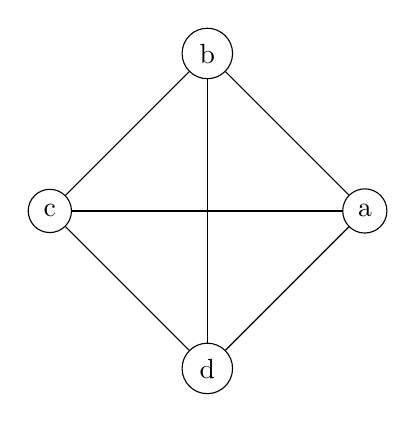
\begin{tikzpicture}
            % Grafo con 4 nodi
            \foreach \nodename/\nodeposition in {a/0, b/90, c/180, d/270}
                \node[circle, draw] (\nodename) at (\nodeposition:2) {\nodename};
            
            \foreach \startnode/\endnode in {a/b, a/c, a/d, b/c, b/d, c/d}
                \draw (\startnode) -- (\endnode);
        \end{tikzpicture}
        \caption{Complete graph with 4 vertices}
        \label{fig:complete_4}
    \end{minipage}%
    \hfill
    \begin{minipage}{0.45\textwidth}
        \centering
        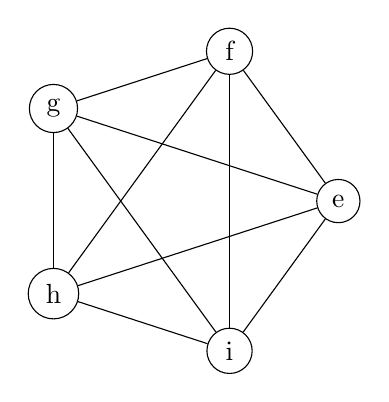
\begin{tikzpicture}
            % Grafo con 5 nodi
            \foreach \nodename/\nodeposition in {e/0, f/72, g/144, h/216, i/288}
                \node[circle, draw] (\nodename) at (\nodeposition:2) {\nodename};
            
            \foreach \startnode/\endnode in {e/f, e/g, e/h, e/i, f/g, f/h, f/i, g/h, g/i, h/i}
                \draw (\startnode) -- (\endnode);
        \end{tikzpicture}
        \caption{Complete graph with 5 vertices}
        \label{fig:complete_5}
    \end{minipage}
\end{figure}

\subsubsection{Bipartite graphs}
If the vertex set of a graph \textit{G} can be split into two disjoint sets \textit{A} and \textit{B} so that each
edge of \textit{G} joins a vertex of \textit{A} and a vertex of \textit{b}, then \textit{G} is a \textbf{bipartite graph}. \\
Alternatively, a bipartite graph is one whose vertices can be coloured black and white in such a way that each edge joins a black vertex (in \textit{A}) and a white vertex (in \textit{B}). \\
Figure \ref{fig:bipartite} is an example of bipartite graph.

\begin{figure}[H]
    \centering
    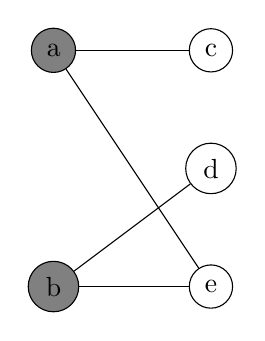
\begin{tikzpicture}[every node/.style={circle, draw, minimum size=0.2cm}]
        % Livello superiore
        \node (A) at (3,0) [fill=black!50] {a};
        \node (B) at (3,-3) [fill=black!50] {b};
        
        % Livello inferiore
        \node (C) at (5,0) [fill=white] {c};
        \node (D) at (5,-1.5) [fill=white] {d};
        \node (E) at (5,-3) [fill=white] {e};
        
        % Collegamenti
        \draw (A) -- (C);
        \draw (A) -- (E);
        \draw (B) -- (D);
        \draw (B) -- (E);
    \end{tikzpicture}
    \caption{}
    \label{fig:bipartite}
\end{figure}



\subsubsection{Bipartite graphs with matching}
A \textbf{bipartite graph with matching} is a bipartite graph in which there is a set of edges selected in such a way that no node is shared among the edges of the matching.
In other words, each node is involved in at most one edge of the matching. \\
This means that if the number of vertices in \textit{A} and \textit{B} is different, at least one vertex will have no connection to another vertex (see Figure \ref{fig:match_1}). \\
If there is the same number of vertices in both \textit{A} and \textit{B}, every vertex is connected to another vertex (see Figure \ref{fig:match_2}). \\
 
\begin{figure}[H]
    \centering
    \begin{minipage}{0.45\textwidth}
        \centering
        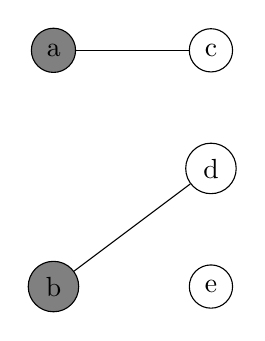
\begin{tikzpicture}[every node/.style={circle, draw, minimum size=0.2cm}]
            % Livello superiore
            \node (A) at (3,0) [fill=black!50] {a};
            \node (B) at (3,-3) [fill=black!50] {b};

            % Livello inferiore
            \node (C) at (5,0) [fill=white] {c};
            \node (D) at (5,-1.5) [fill=white] {d};
            \node (E) at (5,-3) [fill=white] {e};

            % Collegamenti
            \draw (A) -- (C);
            \draw (B) -- (D);
        \end{tikzpicture}
        \caption{}
        \label{fig:match_1}
    \end{minipage}
    \hfill
    \begin{minipage}{0.45\textwidth}
        \centering
        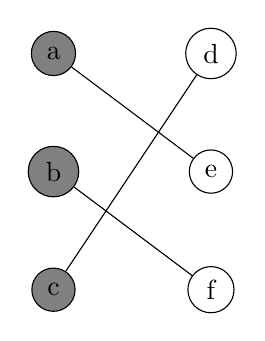
\begin{tikzpicture}[every node/.style={circle, draw, minimum size=0.2cm}]
            % Livello superiore
            \node (A) at (3,0) [fill=black!50] {a};
            \node (B) at (3,-1.5) [fill=black!50] {b};
            \node (C) at (3,-3) [fill=black!50] {c};

            % Livello inferiore
            \node (D) at (5,0) [fill=white] {d};
            \node (E) at (5,-1.5) [fill=white] {e};
            \node (F) at (5,-3) [fill=white] {f};

            % Collegamenti
            \draw (A) -- (E);
            \draw (B) -- (F);
            \draw (C) -- (D);
        \end{tikzpicture}
        \caption{}
        \label{fig:match_2}
    \end{minipage}
\end{figure}


\subsection{Game theory}
Game theory is a type of decision theory in which one’s choice of action is determined after taking
into account all possible alternatives available to an opponent playing the same game, rather than just
by the possibilities of several outcome results. \\
Game theory does not insist on how a game should be played but tells the procedure and principles by which action should be selected.
Thus it is a decision theory useful in competitive situations. \\
Game is defined as an activity between two or more persons according to a set of rules at the end of
which each person receives some benefit or suffers loss. The set of rules defines the game.
Going through the set of rules once by the participants defines a play.
\\

The following sections contains notations and properties accordind to \cite{game_theory:2020}.

\subsubsection{Properties of a Game}
\begin{enumerate}
    \item {There are finite numbers of competitors called \textit{players}.}
    \item {Each player has a finite number of possible courses of action called \textit{strategies}.}
    \item {All the strategies and their effects are known to the players but player does not know which
    strategy is to be chosen.}
    \item {A game is played when each player chooses one of his strategies. The strategies are assumed
    to be made simultaneously with an outcome such that no player knows his opponents strategy
    until he decides his own strategy.}
    \item {The game is a combination of the strategies and in certain units which determines the gain or
    loss.}
    \item {The figures shown as the outcomes of strategies in a matrix form are called \textit{pay-off matrix}.}
    \item {The player playing the game always tries to choose the best course of action which results in
    optimal pay off called \textit{optimal strategy}.}
    \item {The expected pay off when all the players of the game follow their optimal strategies is
    known as \textit{value of the game}. The main objective of a problem of a game is to find the value
    of the game.}
    \item {The game is said to be \textit{fair} game if the value of the game is zero otherwise it's known as \textit{unfair}.}
    \item {A \textit{coalition} is a subset of the players \textit{n}, whereas a \textit{grand coalition} is the
        set \textit{n} of all players. The purpose of a coalition is to coordinate strategies and divide the
        total payoff among all the players.}
\end{enumerate}


\subsubsection{Cooperative Games}
A cooperative game is a situation in which players interact together to achieve a common goal.
In the context of a cooperative game, players aim to maximize the overall outcome by collaborating, communicating, and coordinating their actions.
The primary objective is to achieve a result in which all players benefit, working together to overcome challenges or issues.


\subsubsection{Non-cooperative Games}
A non-cooperative game is a situation in which players act independently and without direct communication or coordination with other players.
In a non-cooperative game, each player seeks to maximize their individual gain without necessarily considering the effect of their actions on other players.
The main goal is to achieve the best personal outcome, even at the expense of other participants, without considering direct collaboration.


\subsubsection{The Prisoner's Dilemma}
The Prisoner's Dilemma is a fundamental concept in game theory that illustrates the challenges of \textit{cooperation} and \textit{non-cooperation} between individuals. \\
It's a model that exemplifies situations where two individuals could benefit from collaboration, but are tempted to act selfishly to maximize their personal gains. \\
Here's how it works:
\\

\textbf{Scenario:}
Imagine two criminals (\textit{A} and \textit{B}) who have been arrested and are held in separate cells. \\
There is not enough evidence to convict them for the most serious crime, but there is enough evidence to convict them for a lesser crime.
Both of them are offered the opportunity to \textit{confess} (\textit{betray}) or \textit{remain silent} (\textit{cooperate}).
\\

\textbf{Options:}
\begin{enumerate}
    \item {If \textit{both remain silent}, they each receive a short sentence of 1 year for the lesser crime.}
    \item {If \textit{one of them betrays} and \textit{the other cooperates}, the betrayer will be released without any sentence, and the other will receive a long sentence of 3 years.}
    \item {If \textit{both betray}, they both receive a moderate sentence of 2 years for the lesser crime, which is longer than if they both cooperate.}
\end{enumerate}

\begin{figure}[H]
    \centering
    \begin{minipage}{0.5\textwidth}
        \centering
        \begin{tabular}{|c|c|c|}
        \hline
        \backslashbox{A}{B} & Silence & Betray \\
        \hline
        Silence & \backslashbox{1}{1} & \backslashbox{3}{0} \\
        \hline
        Betray & \backslashbox{0}{3} & \backslashbox{2}{2} \\
        \hline
        \end{tabular}
        \caption{Years for crimanal \textit{A} and \textit{B}}
        \label{tab:contingency_table_1}
    \end{minipage}%
    \begin{minipage}{0.5\textwidth}
        \centering
        \begin{tabular}{|c|c|c|}
        \hline
        \backslashbox{A}{B} & Silence & Betray \\
        \hline
        Silence & 2 & 3 \\
        \hline
        Betray & 3 & 4 \\
        \hline
        \end{tabular}
        \caption{Total years for the group of criminals}
        \label{tab:contingency_table_2}
    \end{minipage}
    \end{figure}
    

\textbf{Outcomes:}
\begin{itemize}[label=\textbullet]
    \item If both act rationally to maximize their own gain, the most likely outcome is that both will betray, leading to a moderate sentence for both. This is the non-cooperative result.
    \item However, if both trust each other and cooperate, they would achieve the best possible outcome for both: the shortest sentence.
\end{itemize}


\textbf{Implications:} The Prisoner's Dilemma demonstrates how even though cooperating would be in their collective interest, the two prisoners might be tempted to betray each other to avoid a longer sentence. \\
This conflict between personal benefit and the common good often leads to suboptimal outcomes. \\
The Prisoner's Dilemma has been extensively studied in psychology, economics, and social sciences and is a crucial example of the challenges of cooperation in human interactions. \\

